\documentclass{article}
\usepackage[utf8]{inputenc}
\usepackage[margin=1in]{geometry}
\usepackage{graphicx}
\usepackage{natbib}
\usepackage{enumitem}
\usepackage{array}
\usepackage{gensymb}
\usepackage{indentfirst}
\graphicspath{ {Images/} }
\usepackage{float}
\usepackage[table,xcdraw]{xcolor}

\title{Physics 111A Fall 2016- Lab 5\\
JFET Circuits II}
\author{Joshua Levy\\Lab Partner: Alex Chuang}
\date{October 1st, 2016, 2016}

\begin{document}

\maketitle

\section{Lab Write Up}
%1
\subsection{Common Source JFET Amplifier}
    See signature page
%2
\subsection{Increased Gain Common Source JFET Amplifier-Large Drain Resistor}
    \begin{figure}[H]
        \centering
        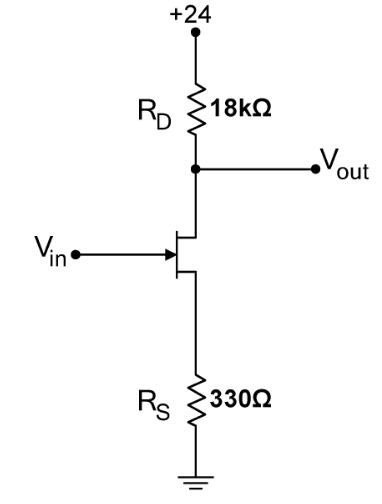
\includegraphics[scale = 0.6]{5_2.png}
        \caption{Increased Gain Common Source JFET Amplifier, Large Drain~\cite{webfig}}
        \label{fig:my_label}
    \end{figure}
    The gain~\cite{webfig}:
    \begin{equation}
        G = V_{out}/V_{in} = -R_D/(R_S+r_s)\approx-R_D/R_S
    \end{equation}
    for [1.1] with an $R_D$ of 1.78k was about 4. Changing the value of $R_D$ to an experimentally measured 18.5k, and $R_S = 0.337k$, and we find that $G = \frac{V_{out}}{V_{in}} = \frac{17.5 mV}{.5 V} \approx 0.035$. This constitutes a substantial drop in gain. We measured the current passing through the resistors, $i_D$ to be 1.38 mA. Matching this current value to the JFET's corresponding $V_{GS}$ on its characteristic curve (lab 4 results), and consequently finding the transconductance for the JFET at that $V_{GS}$ value, and we note by inspection that the transconductance is much lower than expected and thus the internal resistance $r_s$ is much larger than expected. We expect a high gain if the transconductance is high, but in this case, we have a low transconductance, so there should be a significant drop in gain, though the gain should not have dropped as much as it should have. We note that $V_{DS}$ measured to be 71 mV. This means that we are analyzing the circuit in the linear regime of the JFET's output characteristic curve, which behaves dissimilarly to the saturated regime (figure 2c).
    \begin{figure}[H]
        \centering
        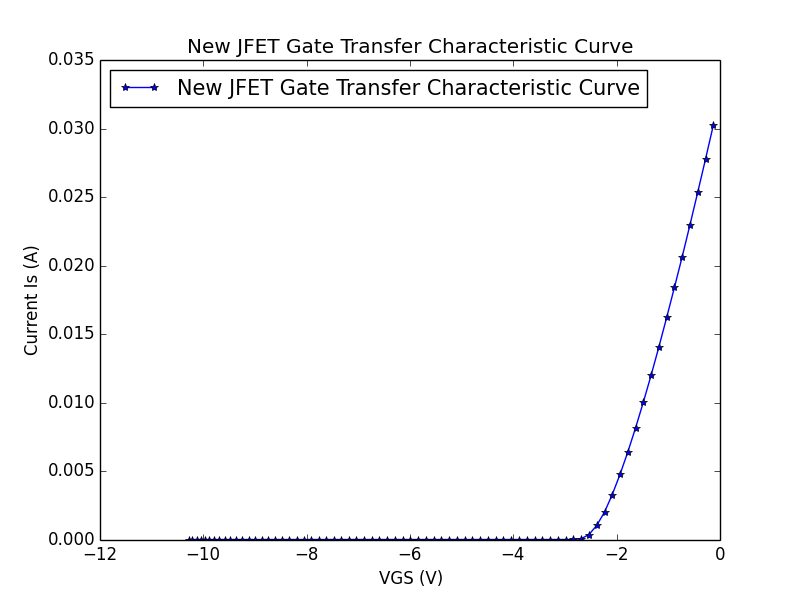
\includegraphics[scale = 0.5]{4_10a.png}
        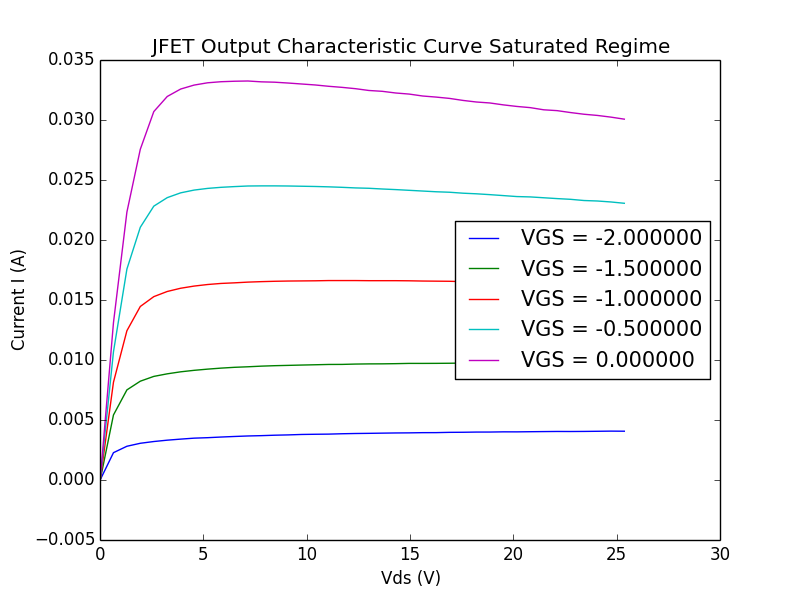
\includegraphics[scale = 0.5]{4_10b.png}
        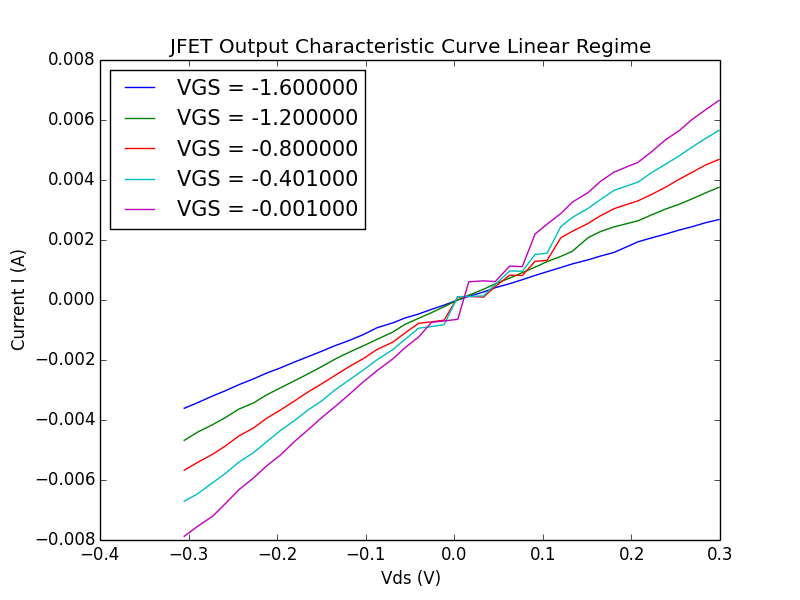
\includegraphics[scale = 0.5]{4_10c.png}
        \caption{New JFET Characteristic Curves (Transfer, saturated output, linear output)}
        \label{fig:my_label}
    \end{figure}
%3
\subsection{Increased Gain Common Source JFET Amplifier-Small Source Resistor}
    \begin{figure}[H]
        \centering
        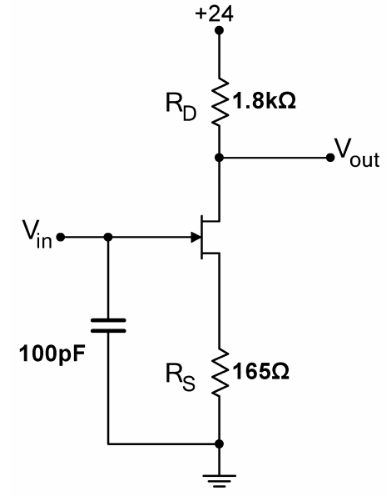
\includegraphics[scale = 0.6]{5_3.png}
        \caption{Increased Gain Common Source JFET Amplifier, Small Source Resistor~\cite{webfig}}
        \label{fig:my_label}
    \end{figure}
    The 100 pF capacitor was measured to be 96.2 pF. $V_{in} = 0.5V$, $V_{out} = 3.6 V$. Thus, our gain for the above circuit is G = $\frac{3.6V}{0.5V} \approx 7.2$. As we change the input amplitude, the maximum undistorted output signal is at 13V for an input signal of 2V. \\\indent After cooling the JFET, we measure $V_{in} = 0.5V$, $V_{out} = 3.92 V$, and find the gain to be 7.84, an increase of 0.64 from its original value. For the four other JFETs, we find the following gain values: 
    \begin{table}[H]
        \centering
        \caption{JFET Amplifier Gain Values}
        \label{my-label}
        \begin{tabular}{ccc}
        \textbf{JFET} & \textbf{Vout (V)} & \textbf{Gain} \\ \hline
        Original & 3.6 & 7.2 \\
        1 & 3.52 & 7.04 \\
        2 & 3.68 & 7.36 \\
        3 & 3.68 & 7.36 \\
        4 & 3.52 & 7.04
        \end{tabular}
    \end{table}
    The gain found in [1.1] was 4. Cooling the JFET increased this gain to 4.25. Thus, the fractional increase in gain after cooling the JFET is $\frac{G_{cool} - G_{regular}}{G_{regular}} \approx 6.25\%$. The gain found in this part is 7.2. The "cooled" gain in this part is 7.82. This leads to an increase of about $8.6\%$. We see that the fractional increase in gain is larger in [1.3] than in [1.1] because looking at eq.(1), we note that cooling will decrease the internal resistance of the JFET $r_s$ by pretty much the same amount for each part. However, the circuit in part [1.3] has a smaller source resistance, so in eq.(1), decreasing $r_s$ has a greater effect on the denominator of eq.(1), thereby increasing the gain even more so when cooled. 
    
%4
\subsection{Increased Gain Common Source JFET Amplifier-Source Resistor Bypass}
    \begin{figure}[H]
        \centering
        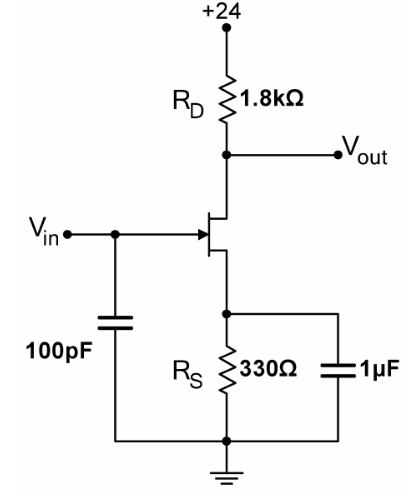
\includegraphics[scale = 0.6]{5_4.png}
        \caption{Increased Gain Common Source JFET Amplifier, Source Resistor Bypass~\cite{webfig}}
        \label{fig:my_label}
    \end{figure}
    We measured the 100 pF capacitor ($C_1$) as 96.2 pF and the 1 $\mu$F capacitor ($C_2$) as 1.04 $\mu$F, and using the values of $R_D = 1.78k$ and $R_S = 0.337k$ from the previous parts. We measured the gain of the above circuit for the following input signal frequencies:
    \begin{table}[H]
        \centering
        \caption{JFET Amplifier Source Resistor Bypass Gain for Various Input Frequencies}
        \label{my-label}
        \begin{tabular}{cccc}
        \textbf{f (Hz)} & \textbf{$V_{in}$ (V)} & \textbf{$V_{out}$ (V)} & \textbf{Gain} \\ \hline
        100 & 0.98 & 4 & 4.081632653 \\
        300 & 0.98 & 4.8 & 4.897959184 \\
        1000 & 0.98 & 8.2 & 8.367346939 \\
        3000 & 0.98 & 13.8 & 14.08163265 \\
        10000 & 0.98 & 15.8 & 16.12244898 \\
        30000 & 0.98 & 16 & 16.32653061 \\
        100000 & 0.98 & 15.8 & 16.12244898
        \end{tabular}
    \end{table}
    We see in the table above that as the frequency increases, the gain increases for the circuit. Thus, the gain is frequency dependent. We can predict the frequency dependence of this gain. Replacing the $R_S$ in eq.(1) with $Z_{eq}$, where $Z_{eq} = \frac{R_S}{jR_S \omega C_2 + 1}$ is the equivalent impedance of $R_S$ and $C_2$ in parallel, and finding the magnitudes of the numerator and denominator using multiplication of complex conjugates, and we attain the predicted gain:
    \begin{equation}
        G_{predicted} = \frac{R_D}{Z_{eq} + r_s} = \frac{R_D R_S j \omega C_2 + R_D}{R_S + r_s + R_S + r_s + R_S r_s j \omega C_2} = \frac{R_D(R_S + r_s) + R_D r_s (R_S\omega C_2)^{2} + j\beta \omega}{(R_S + r_s)^{2} + (R_S r_s \omega C_2)^{2}}
    \end{equation}
    where $\omega$ is two times the input signal frequency, f, $r_s$ is the internal resistance of the JFET, and j is an imaginary number. We find the approximate internal resistance of the JFET using a load line analysis on the intersection between the curve $i_D = \frac{-V_{GS}}{R_S}$ and the characteristic curve to find the equilibrium $V_{GS}$ value. A $V_{GS}$ value of -1.54 V was found via graphical analysis (figure 5). We use the $V_{GS}$ to search for internal resistance using interpolation of internal resistance data points, we find $r_s$ to be $\approx 82\Omega$. Taking the limit of the predicted gain as $\omega \rightarrow \infty$, and we see that the gain changes to $G_p \approx \frac{R_D}{r_s}$. Plugging in $R_D$ and $r_s$, and we attain a predicted gain of 21.7, which is about 25.3$\%$ off from our measured value.\\\indent We notice that the source impedance ($Z_{eq}$) is decreased by the use of a capacitor in parallel to the source resistor. Thus, a decrease in source impedance from inserting the capacitor $C_2$ increases the gain of the amplifier.
    \begin{figure}[H]
        \centering
        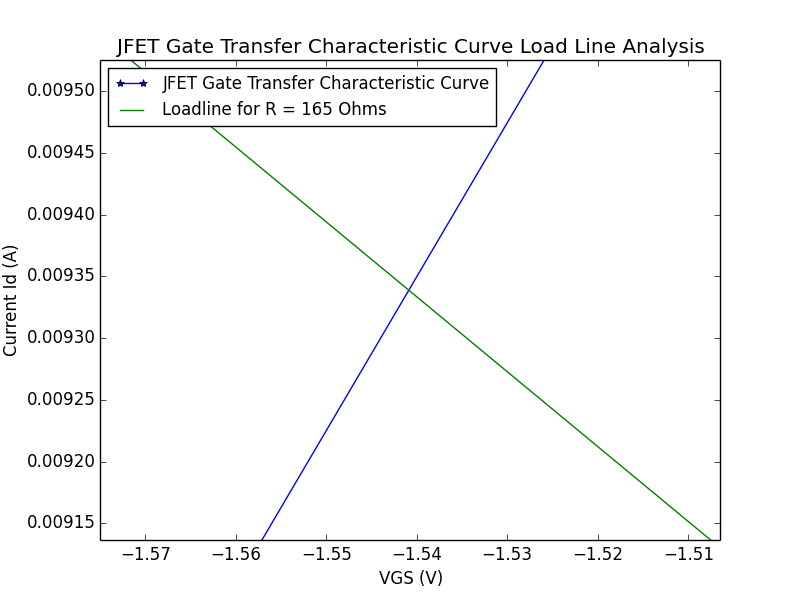
\includegraphics[scale = 0.5]{5_4b.png}
        \caption{Load Line Analysis for R = 165 Ohms}
        \label{fig:my_label}
    \end{figure}
%5
\subsection{Differential Amplifier}
    See signature page.
%6
\subsection{Improved Diffential Amplifier}
    See signature page.
%7
\subsection{JFET Attenuator}
    \begin{figure}[H]
        \centering
        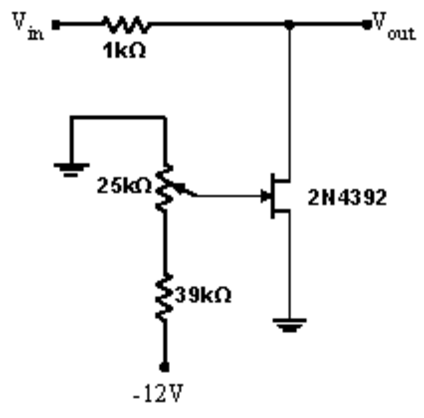
\includegraphics[scale = 0.6]{5_7.png}
        \caption{JFET Attenuator~\cite{webfig}}
        \label{fig:my_label}
    \end{figure}
    \begin{figure}[H]
        \centering
        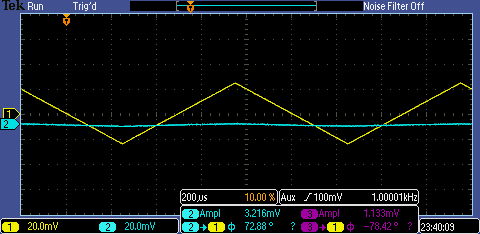
\includegraphics[scale = 0.5]{TEK00000.PNG}
        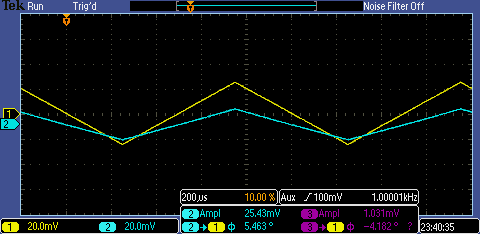
\includegraphics[scale = 0.5]{TEK00001.PNG}
        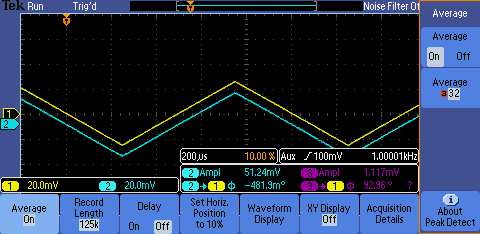
\includegraphics[scale = 0.5]{tek00002.PNG}
        \caption{Varying the Output Amplitude with the Potentiometer}
        \label{fig:my_label}
    \end{figure}
    Figure 7 demonstrates out ability to vary the output amplitude $V_{out}$ with the potentiometer for the given attenuator circuit (figure 6) and a $V_{in}$ of 0.05 V triangle wave. We see that the circuit is still linear in this case, maintaining the triangle wave shape, and the output ranges from 0 V to the amplitude of the input. We adjusted the potentiometer until the gain for the circuit was 0.5, then increased the input voltage until we found our first distorted output signal, which occurred when $V_{in} = 204 mV$. The circuit is no longer linear at this point. 
    
%8
\subsection{Linearized JFET Attenuator}
    \begin{figure}[H]
        \centering
        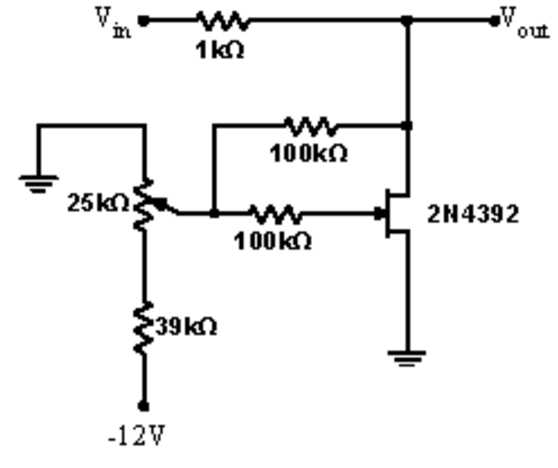
\includegraphics[scale = 0.6]{5_8.png}
        \caption{Linearized JFET Attenuator~\cite{webfig}}
        \label{fig:my_label}
    \end{figure}
    In the circuit above, we measure the following resistance values using the LCR meter:\\
    $R_{1k} = 1.006k$\\
    $R_{39k} = 43.2k$\\
    $R_{100k} = 100.1k$\\
    $R_{100k} = 100.2k$\\\indent Once we set the potentiometer to a value such that the gain is 0.5, we increased $V_{in}$ until we found the largest undistorted output signal, which is when $V_{in} = 420 mV$, an amplitude of about twice that of the previous section.\\\indent For a $V_{in}$ value of 96.7 mV, we set the potentiometer so that we attain the maximum attenuation. For this, $V_{out}$ was measured to be 4.0 mV, yielding a gain of 0.0414.\\\indent In calculating the JFET drain-source resistance $R_{DS}$ we utilize the linear relation ~\cite{webfig}:
    \begin{equation}
        \frac{1}{R_{DS}} = 2k[(V_{GS}-V_P)-V_{DS}/2]
    \end{equation}
    where $V_P$ is the pinchoff point where the JFET begins conducting, (i.e. the point on the JFET transfer characteristic curve where $i_D$ is close to 0). And using the relation ~\cite{lecture}:
    \begin{equation}
        k = \frac{I_{dss}}{V_P^{2}}
    \end{equation}
    where $I_{dss}$ is the $i_D$ current value where $V_{GS} = 0$. And the estimating that $V_{GS} \rightarrow 0$ because a reducing the potentiometer impedance to $0\Omega$ substantially decreases the magnitude of the gate voltage so that the gate voltage is a small negative value. Assuming that we are considering the linear region of the JFET $V_{DS}$ $i_{D}$ output characteristic curve to make such a fit, we also assume that $V_{DS}$ is close to 0.\\\indent Using my JFET's characteristic curves, and fitting the polynomial approximation curve found in lab 4:
    \begin{equation}
        i_D(V_{GS}) = 0.0025V_{GS}^{2} + 0.0193V_{GS} + 0.0332
    \end{equation}
    to the data points, $I_{dss} \approx 0.0332 A$, and $V_P \approx -2.59 V$. Plugging this into eq.(3), we find that:
    \begin{equation}
        R_{DS} = \frac{-1}{2(\frac{I_{dss}}{V_P^{2}}) V_P} = \frac{-V_P}{2 I_{dss}} = \frac{2.59 V}{2*0.0332 A} \approx 39 \Omega
    \end{equation}
    Our actual $R_{DS}$ is found from the voltage divider relation $G = \frac{R_{DS}}{1.006k + R_{DS}}$. Given that G = 0.0414, and rearranging the voltage divider relation, we find our empirical $R_{DS}$:
    \begin{equation}
        R_{DS} = \frac{1.006k * G}{1 - G} \approx 43.44 \Omega
    \end{equation}
    which is really close to the theoretical $R_{DS}$ calculated above. This verifies our results.
%9
\subsection{JFET Modulator}
    \begin{figure}[H]
        \centering
        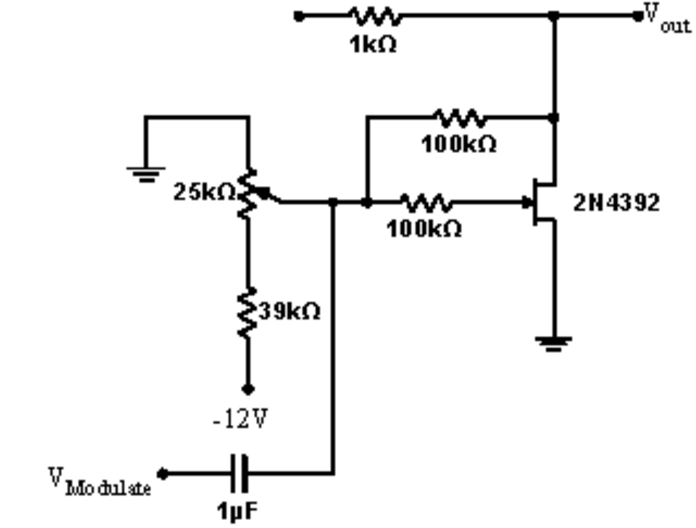
\includegraphics[scale = 0.6]{5_9.png}
        \caption{JFET Modulator~\cite{webfig}}
        \label{fig:my_label}
    \end{figure}
    \begin{figure}[H]
        \centering
        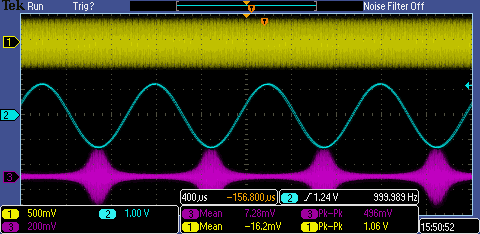
\includegraphics[scale = 0.6]{tek00003.PNG}
        \caption{Scope Trace of JFET Modulator}
        \label{fig:my_label}
    \end{figure}
    Building the circuit depicted in figure 9 and measuring the new 1 pF capacitor to be 980.5 nF, we attain the above scope trace of the modulated circuit driving $V_{modulate}$ and $V_{in}$ with the specified parameters mentioned in the lab sheet.
%10
\subsection{JFET AM Transmitter}
    See signature page
%11
\subsection{Surprise Circuit}
    \begin{figure}[H]
        \centering
        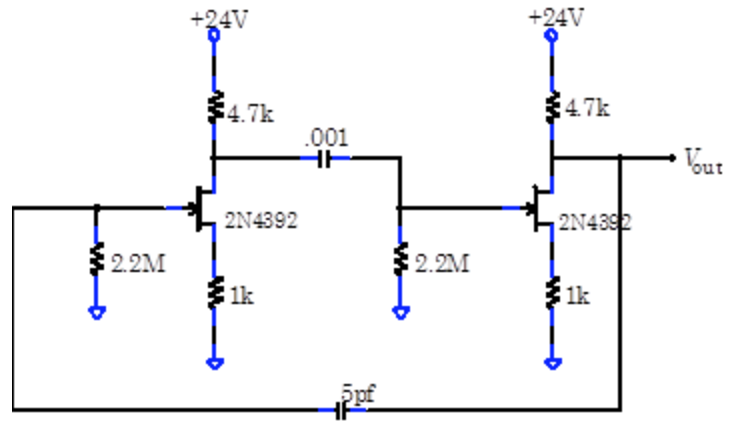
\includegraphics[scale = 0.7]{5_11.png}
        \caption{Surprise Circuit~\cite{webfig}}
        \label{fig:my_label}
    \end{figure}
    \begin{figure}[H]
        \centering
        
            A) 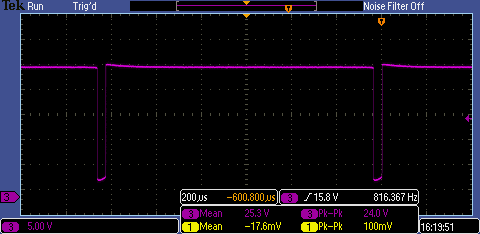
\includegraphics[scale = 0.5]{TEK00004.PNG}\\
            B) 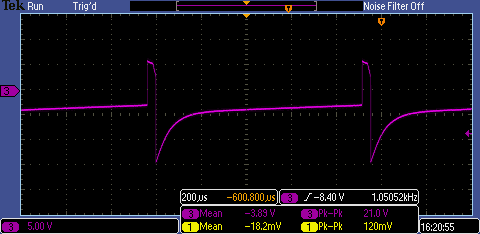
\includegraphics[scale = 0.5]{TEK00005.PNG}\\
            C) 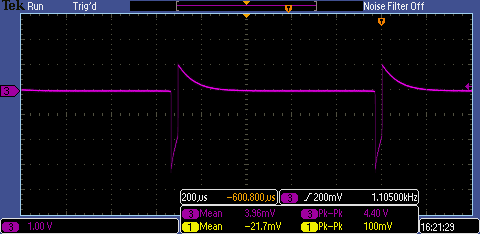
\includegraphics[scale = 0.5]{tek00006.PNG}
        
        \caption{Surprise Circuit Scope Traces: A) $V_{out}$ B) input of right JFET and C) input of left JFET}
        \label{fig:my_label}
    \end{figure}
    We built the surprise circuit (figure 11) and noticed that it outputs an inverted pulse at regular intervals (figure 12A). The output of the circuit travels to the bottom capacitor (5pF) and since the 5 pF capacitor and the 2.2M resistor make up a high pass filter, the output has lost its DC dependence. We notice that this capacitor (5pF) has small capacitance and is discharging in this scenario. It spends a really short time doing so. This signal is fed into the left JFET (figure 12C). The left JFET amplifies this signal, inverts it, and passes it into a high pass filter formed by 0.001 $\mu$F capacitor at the top and the 2.2M resistor, and this signal passes through to the right JFET (figure 12B). We note that the 0.001 $\mu$F capacitor is charged for a short period of time and then more slowly discharges than the 5pF capacitor. We see that any low pass/DC dependence has been cut off once more as it passes to the right JFET. The right JFET inverts and amplifies this signal, producing the output image we see in figure 12A. What is happening is that the output pulse charges the 5pF capacitor, and then as it discharges, the 0.001 $\mu$F capacitor successively charges then discharges. The successive charging and discharging of the capacitors results in the production of the output.\\ We measured the following values for each circuit component:\\
    $R_{4k1}$ = 4.68k\\ 
    $R_{4k2}$ = 4.70k\\ 
    $R_{1k1}$ = 0.986k\\ 
    $R_{1k2}$ = 0.996k\\ 
    $R_{2M1}$ = 2.15M\\ 
    $R_{2M2}$ = 2.17M\\ 
    $C_{5p}$ = 5.05 pF\\
    $C_{0.001\mu}$ = 1 nF
    
%12
\subsection{Phase Splitter}
    \begin{figure}[H]
        \centering
        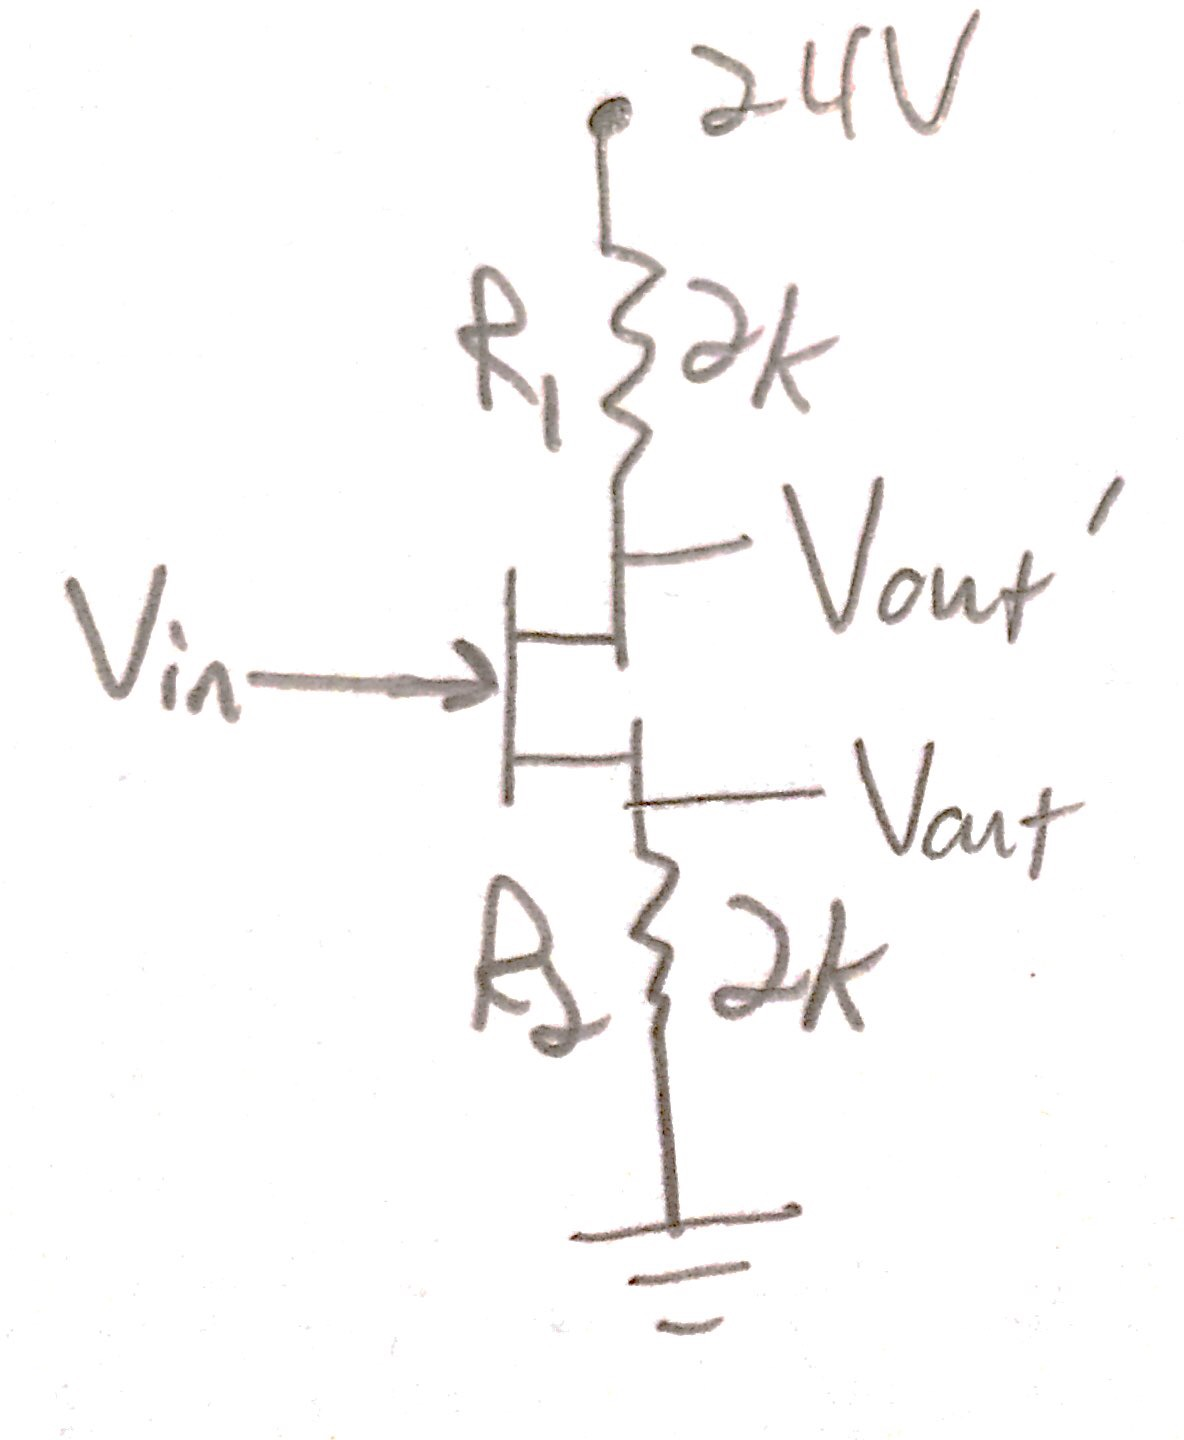
\includegraphics[scale = 0.15]{IMG2.JPG}
        \caption{Design of Phase Splitter}
        \label{fig:my_label}
    \end{figure}
    The phase splitter was designed by making a symmetric circuit with $R_D = R_1 = R_2 = R_S = 2k$, and outputting a signal directly above ($V_{out}'$, which is in the drain) and below the JFET ($V_{out}$, which is in the source). Matching the resistor values approximately will cause the magnitude gains to essentially match and be near unity, and setting the larger resistor value of 2k assures that the effect of the transconductance is closer to being negligible in finding our gain. We would expect $V_{out}'$ to be the 180$\degree$ phase shifted signal and $V_{out}$ to be the non phase shifted signal. We measured $R_1 = 1.96k$ and $R_2 = 2.02k$. When we put this circuit to the test with a $V_{in}$ of 404 mV, we measured $V_{out}'$ to be 348 mV with a 170 $\degree$ phase shift and $V_{out}$ to be 396 mV, which is the effect we expect. The internal resistance of the JFET is probably responsible for any discrepancies. We increased the amplitude of the phase splitter and found that the largest distorted output signal is at 5.4V.

%13
\subsection{High Gain Amplifier}
    \begin{figure}[H]
        \centering
        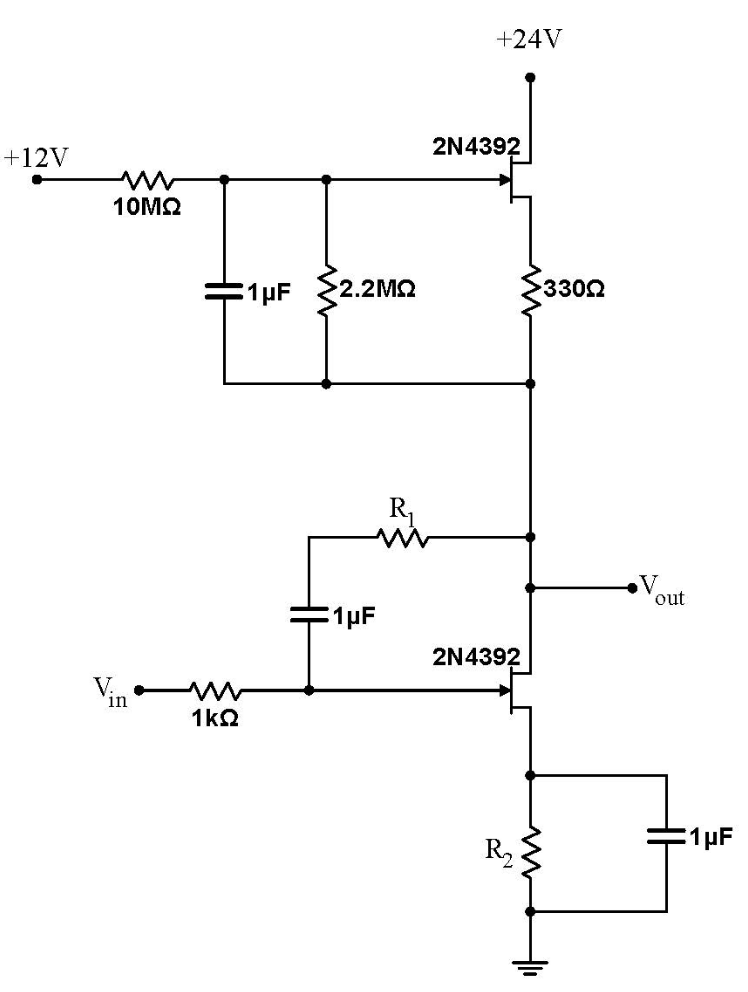
\includegraphics[scale = 0.6]{5_13.png}
        \caption{High Gain Amplifier~\cite{webfig}}
        \label{fig:my_label}
    \end{figure}
    When constructing the circuit above, we measured the 10M resistor to be 10.12M, the upper 330$\Omega$ resistor as 0.329k, the upper $1 \mu$F capacitor as 0.958 $\mu$F, the 2.2k resistor as 2.16k, the middle $1 \mu$F capacitor as 1.02 $\mu$F, the 1k resistor as 1.039k, and the bottom $1 \mu$F capacitor as 0.98 $\mu$F. We found and used $R_1$ (33k) of 34.1k and $R_2$ (330$\Omega$) of 0.339k. \\\indent
    In order to make the circuit symmetric and have similar voltage drops across the JFETs, the $R_2$ value of 0.339k was chosen, which matches the upper 330$\Omega$ resistor. Without $R_1$ put into the circuit, we attained the following gains with a 20 mV input signal:
    \begin{table}[H]
        \centering
        \caption{Gain of High Gain Amplifier, Various Frequencies, No $R_1$}
        \label{my-label}
        \begin{tabular}{llll}
        \textbf{f (Hz)} & \textbf{Vin (V)} & \textbf{Vout (V)} & \textbf{Gain} \\ \hline
        100 & 0.02 & 2.3 & 115 \\
        1k & 0.02 & 3.2 & 160 \\
        10k & 0.018 & 3.5 & 194.4444444 \\
        100k & 0.02 & 1.4 & 70 \\
        1M & 0.02 & 0.145 & 7.25 \\
        19.4k & 0.02 & 3.16 & 158
        \end{tabular}
    \end{table}
    90$\%$ gains were found at frequencies of 1kHz and 19.4kHz. The output peaked at 5.4kHz frequency with $V_{in} = 20mV$ and $V_{out} = 3.53V$. Setting $V_{in}$ to the $f_{peak}$ of 5.4kHz, we measure the gain for other JFETs inserted instead of the lower JFET:
    \begin{table}[H]
        \centering
        \caption{Gain of High Gain Amplifier, Various JFETs, No $R_1$}
        \label{my-label}
        \begin{tabular}{llll}
        \textbf{Other JFET} & \textbf{Vin (V)} & \textbf{Vout (V)} & \textbf{Gain} \\ \hline
        1 & 0.02 & 3.28 & 164 \\
        2 & 0.02 & 2.52 & 126 \\
        3 & 0.02 & 4.12 & 206
        \end{tabular}
    \end{table}
    The gain is not independent of the JFET. Inputting a square wave to the original JFET, and we attain the following output scope trace:\\
    \begin{figure}[H]
        \centering
        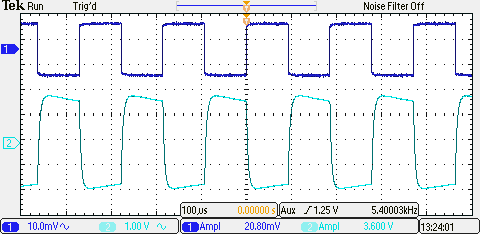
\includegraphics[scale = 0.7]{TEK00007.PNG}
        \caption{Output Scope Trace of Square Wave Passing Through High Gain Amplifier, No $R_1$}
        \label{fig:my_label}
    \end{figure}
    Returning to the sine wave, we cool the lower JFET. Before cooling, the output gain is $\frac{V_{out}}{V_{in}} = \frac{3.53V}{0.020V} \approx 176.5$. After cooling, the output voltage is 3.8V, and the gain is 190. The gain increased by approximately 13.5 after cooling.\\\indent 
    Now we add $R_1$, and  we attained the following gains with a 20 mV input signal:
    \begin{table}[H]
        \centering
        \caption{Gain of High Gain Amplifier, Various Frequencies, With $R_1$}
        \label{my-label}
        \begin{tabular}{llll}
        \textbf{f (Hz)} & \textbf{Vin (V)} & \textbf{Vout (V)} & \textbf{Gain} \\ \hline
        100 & 0.02 & 0.381 & 19.05 \\
        1k & 0.02 & 0.472 & 23.6 \\
        10k & 0.0192 & 0.496 & 25.83333333 \\
        100k & 0.019 & 0.456 & 24 \\
        1M & 0.0196 & 0.133 & 6.785714286 \\
        700 & 0.0196 & 0.453 & 23.1122449
        \end{tabular}
    \end{table}
    90$\%$ gains were found at frequencies of 700Hz and 100kHz. The output peaked at 5.4kHz frequency with $V_{in} = 20mV$ and $V_{out} = 0.500V$. Setting $V_{in}$ to the $f_{peak}$ of 5.4kHz, we measure the gain for other JFETs inserted instead of the lower JFET:
    \begin{table}[H]
        \centering
        \caption{Gain of High Gain Amplifier, Various JFETs, With $R_1$}
        \label{my-label}
        \begin{tabular}{llll}
        \textbf{Other JFET} & \textbf{Vin (V)} & \textbf{Vout (V)} & \textbf{Gain} \\ \hline
        1 & 0.0196 & 0.452 & 23.06122449 \\
        2 & 0.0196 & 0.433 & 22.09183673 \\
        3 & 0.0196 & 0.472 & 24.08163265
        \end{tabular}
    \end{table}
    The gain is not independent of the JFET. Inputting a square wave to the original JFET, and we attain the following output scope trace:\\
    \begin{figure}[H]
        \centering
        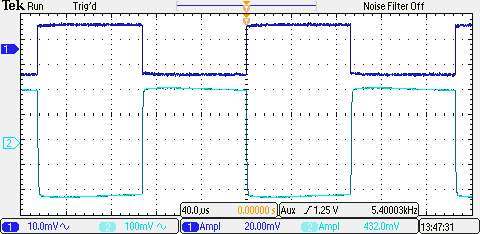
\includegraphics[scale = 0.7]{TEK00009.PNG}
        \caption{Output Scope Trace of Square Wave Passing Through High Gain Amplifier, With $R_1$}
        \label{fig:my_label}
    \end{figure}
    We notice that the output of the square wave input for this circuit is more rigid and square than the output of the circuit without $R_1$.
    \\\indent Returning to the sine wave, we cool the lower JFET. Before cooling, the output gain is $\frac{V_{out}}{V_{in}} = \frac{0.5V}{0.020V} \approx 25$. After cooling, the output voltage is 0.512V, and the gain is 25.6. The gain increased by approximately 0.6 after cooling. Thus, the circuit is much less sensitive to temperature changes than the circuit without $R_1$.
%14
\subsection{High Gain Amplifier Explanation}
    \begin{figure}[H]
        \centering
        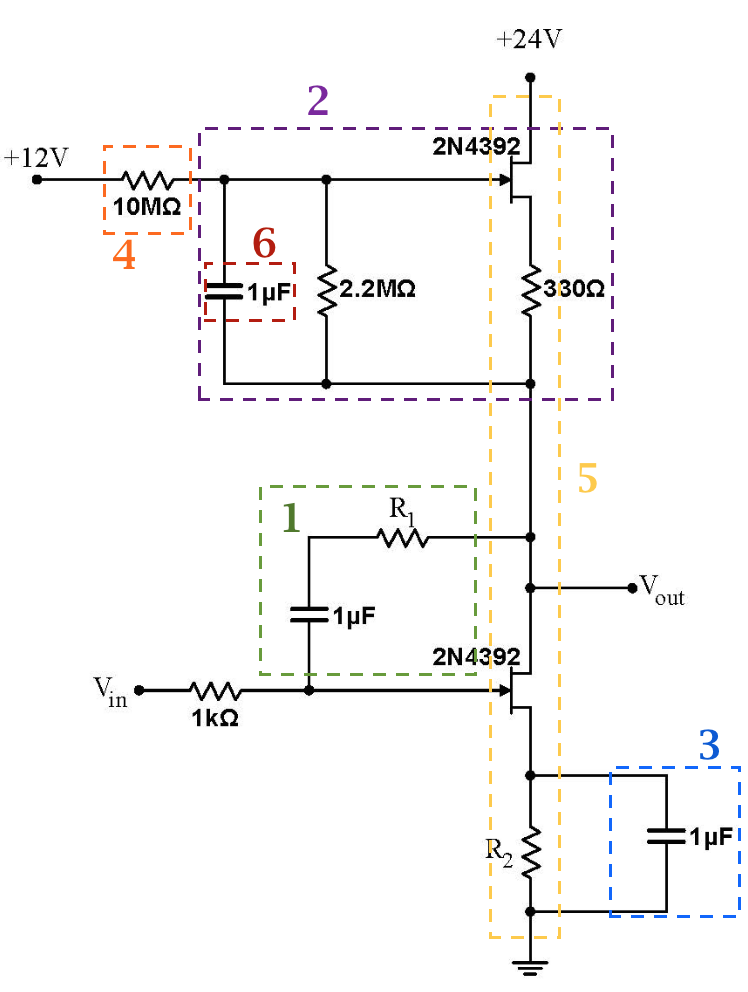
\includegraphics[scale = 0.7]{5_14.png}
        \caption{High Gain Amplifier Color Labelled for [1.14]~\cite{webfig}}
        \label{fig:my_label}
    \end{figure}
    Referring to the above figure, we make the following assertions about the function of the circuit components (note that each list number corresponds to a part of the circuit that is colored and labelled by that number to reduce ambiguity):
    \begin{enumerate}
        \item The $R_1$ resistor in series with the 1 $\mu$F capacitor sets the gain of the circuit through feedback, because the voltage drop across the two elements is registered by a drop in $V_{GS}$ of the second transistor which in turn slightly changes the current in the main right side of the circuit (yellow 5 part). As this current decreases,the voltage drops across the two elements decrease, thereby increasing $V_{GS}$ and the current and this feedback process continues until an equilibrium point is reached. The gain is directly proportional to the output voltage of the amplifier, which in turn is proportional to the current passing through the right side of the circuit, which is altered by the feedback produced from the green circuit part 1.
        \item The purple circuit part 2, that is, the 330$\Omega$ and 2.2M resistors, the 1 $\mu$F capacitor and JFET in the upper leg of the circuit function as a current source. The current source has a very high stiffness in the saturated regime, and using the current source as the drain resistance $R_D$ of the amplifier in the lower leg, the current source will increase the gain.
        \item The blue-labeled (circuit part 3) 1 $\mu$F capacitor that is in parallel to the source resistor $R_2$ bypasses the source resistor and increases the open-loop gain. This occurs because we can consider $R_2$ and the capacitor $C_3$ in series to have an equivalent impedance of $Z_{eq} = \frac{R_2 * Z_{C_3}}{R_2 + Z_{C_3}}$. $Z_{eq}$ functions as the new source resistor, and thus the new gain of the circuit is approximated by:
        \begin{equation}
            G_{approx} \approx \frac{R_D}{Z_{eq}}
        \end{equation}
        $Z_{C_3}$ is inversely proportional to the frequency $\omega$ of the incoming signal carried by the current $i_D$ and capacitance $C_3$. Assuming that $\omega$ is very large, we see that $Z_{eq}$ drops to a low value, thereby significantly increasing the open-loop gain. The capacitor dominates/ significantly reduces this impedance necessary for large increases in gain in this case.
        \item The 10M resistor, orange circuit part 4, is probably responsible for setting the current through the JFETs because most of the $V_{GS}$ for the upper JFET is determined by the voltage drop across that resistor. We see that most of the voltage is dropped by the 10M, and thus, $V_{GS}$ is significantly modified/lowered, much more than the $V_{GS}$ in the lower JFET. Thus, the upper JFET, will constrict the flow of current passing through the circuit much more than the lower JFET and the upper JFET's gate is largely controlled by the 10M resistor. So the 10M resistor is mostly responsible for setting the current $i_D$ through the JFETS.
        \item If we do not look at the left side of the circuit, or only look at the combinations of circuit elements inside yellow circuit part 5, and considering that the source resistance $R_2$ of the lower JFET is approximately equal to the source resistance of 330$\Omega$ of the upper JFET, and considering that the JFETs are matched, by symmetry (or treating each JFET and source resistor as one resistor, and treating the whole system as a voltage divider), we would expect that there would be similar voltage drops across each JFET. So the fact that $R_2$ is approximately the same source resistance of the upper JFET, we experience similar voltage drops.
        \item The 1 $\mu$F capacitor $C_1$ of red circuit part 6 increases the stiffness of the current source by bypassing AC signals. The 10M resistor and $C_1$ appear to form a high pass filter, thus lower frequency and DC signals do not pass through as well. In this case, we find that mostly AC signals pass through the divider near circuit parts 4 and 6. The voltage coming out of the junction between circuit parts 4 and 6 is essentially the voltage output of a highpass AC bypass filter.
    \end{enumerate}
%15
\subsection{Improved Differential Amplifier Gain}
    \begin{figure}[H]
        \centering
        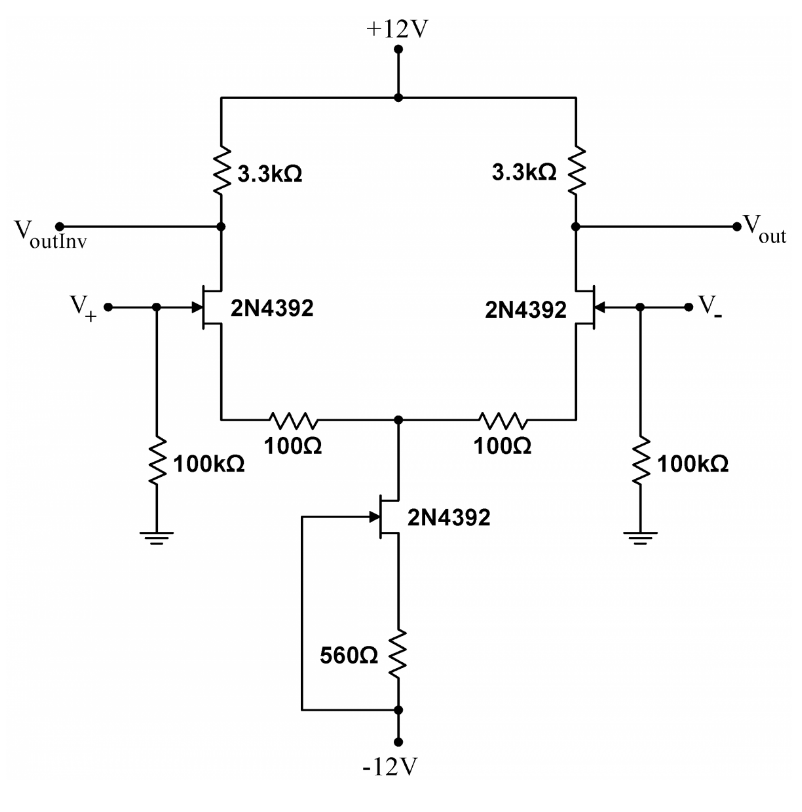
\includegraphics[scale = 0.6]{5_15.png}
        \caption{Improved Differential Amplifier ~\cite{webfig}}
        \label{fig:my_label}
    \end{figure}
    We note that the common mode gain is ~\cite{webfig}:
    \begin{equation}
        G_C = \frac{R_D}{2R_1 + R_S + r_s}
    \end{equation} 
    and the differential gain is ~\cite{webfig}:
    \begin{equation}
        G_{\Delta} = \frac{R_D}{R_S + r_s}
    \end{equation}
    We note that for using a self-biased current source, we assume $R_1$ to have large stiffness, which we found in the last lab to be $\approx 200000 \Omega$. In [1.6], with an $R_D$ of 3.3k, and choosing $R_1$ to be the stiffness of 200000 $\Omega$, we can thus estimate the common mode gain to be:
    \begin{equation}
        G_C \approx \frac{R_D}{2R_1} = \frac{3.3k}{400k} \approx 0.00825
    \end{equation} 
    When we took our actual measurements for the common gain, $V_{in} = 52 mV$ and $V_{out} = 5.8 mV$, so the actual common gain we measured was $\approx 0.112$, which is roughly on a similar order of magnitude as our predicted common mode gain.
    \\\indent For the differential gain, we assume $R_D$ to be the same value, $R_S = 100 \Omega$, and doing a load line analysis on the self-biased current source under the assumption that the JFET characteristic curve of the JFET in the current source is similar to the two matching JFETs' curves.
    \begin{figure}
        \centering
        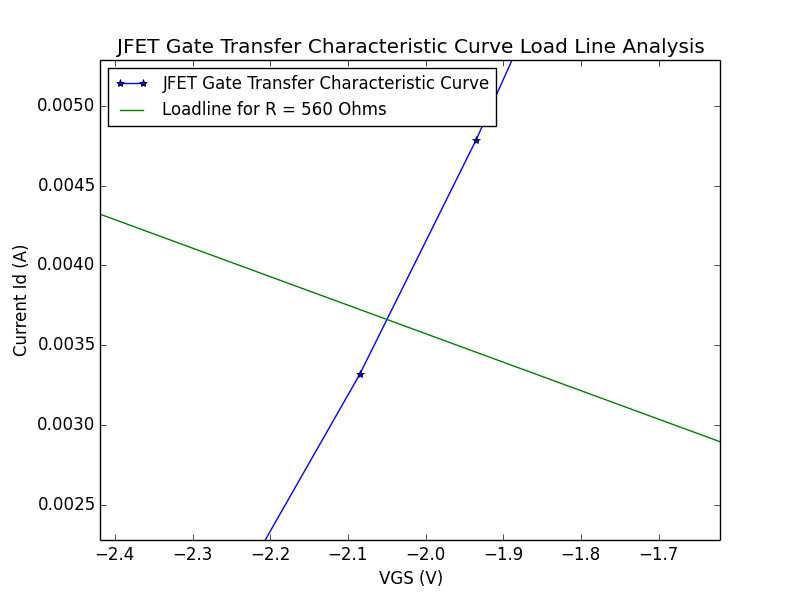
\includegraphics[scale = 0.5]{5_15b.png}
        \caption{Load Line Analysis Self-Biased Current Source of Differential Amplifier}
        \label{fig:my_label}
    \end{figure}
    This graphical analysis yields the current of 3.667 mA flowing through the common bottom part of the differential amplifier. This current, I, can be divided into I = $i_L + i_R$, where the currents come from the left and right sides of the differential amplifier respectively and join at the bottom. And we estimate due to symmetry that half the current flows in each side (in all actuality this is not true, but it gives us an idea of finding $r_s$). Matching a current of 1.83 mA to the JFET curve of one of the left or right top JFETs, and we get a $V_{GS}$ of -2.27 V, corresponding to an $r_s$ internal resistance value of $\approx 172 \Omega$. Plugging these values into eq.(10) and our predicted differential gain is:
    \begin{equation}
        G_{\Delta P} = \frac{3.3k}{100 \Omega + 172 \Omega} \approx 12.13
    \end{equation}
    In actuality, we measured $V_{in}$ or $V_{+}$ to be 52 mV, $V_{-} = 0 mV$, yielding $V_{\Delta} = \frac{V_+ - V_-}{2} = 26 mV$ and $V_{out}$ to be 270 mV yielding the actual gain of $G = \frac{V_{out}}{V_{\Delta}} = \frac{270 mV}{26 mV} \approx 10.38$, which is quite close to our predicted value of 12.13, only off by 14$\%$.
    
%end


\section{Signature Page}
\begin{center}
    $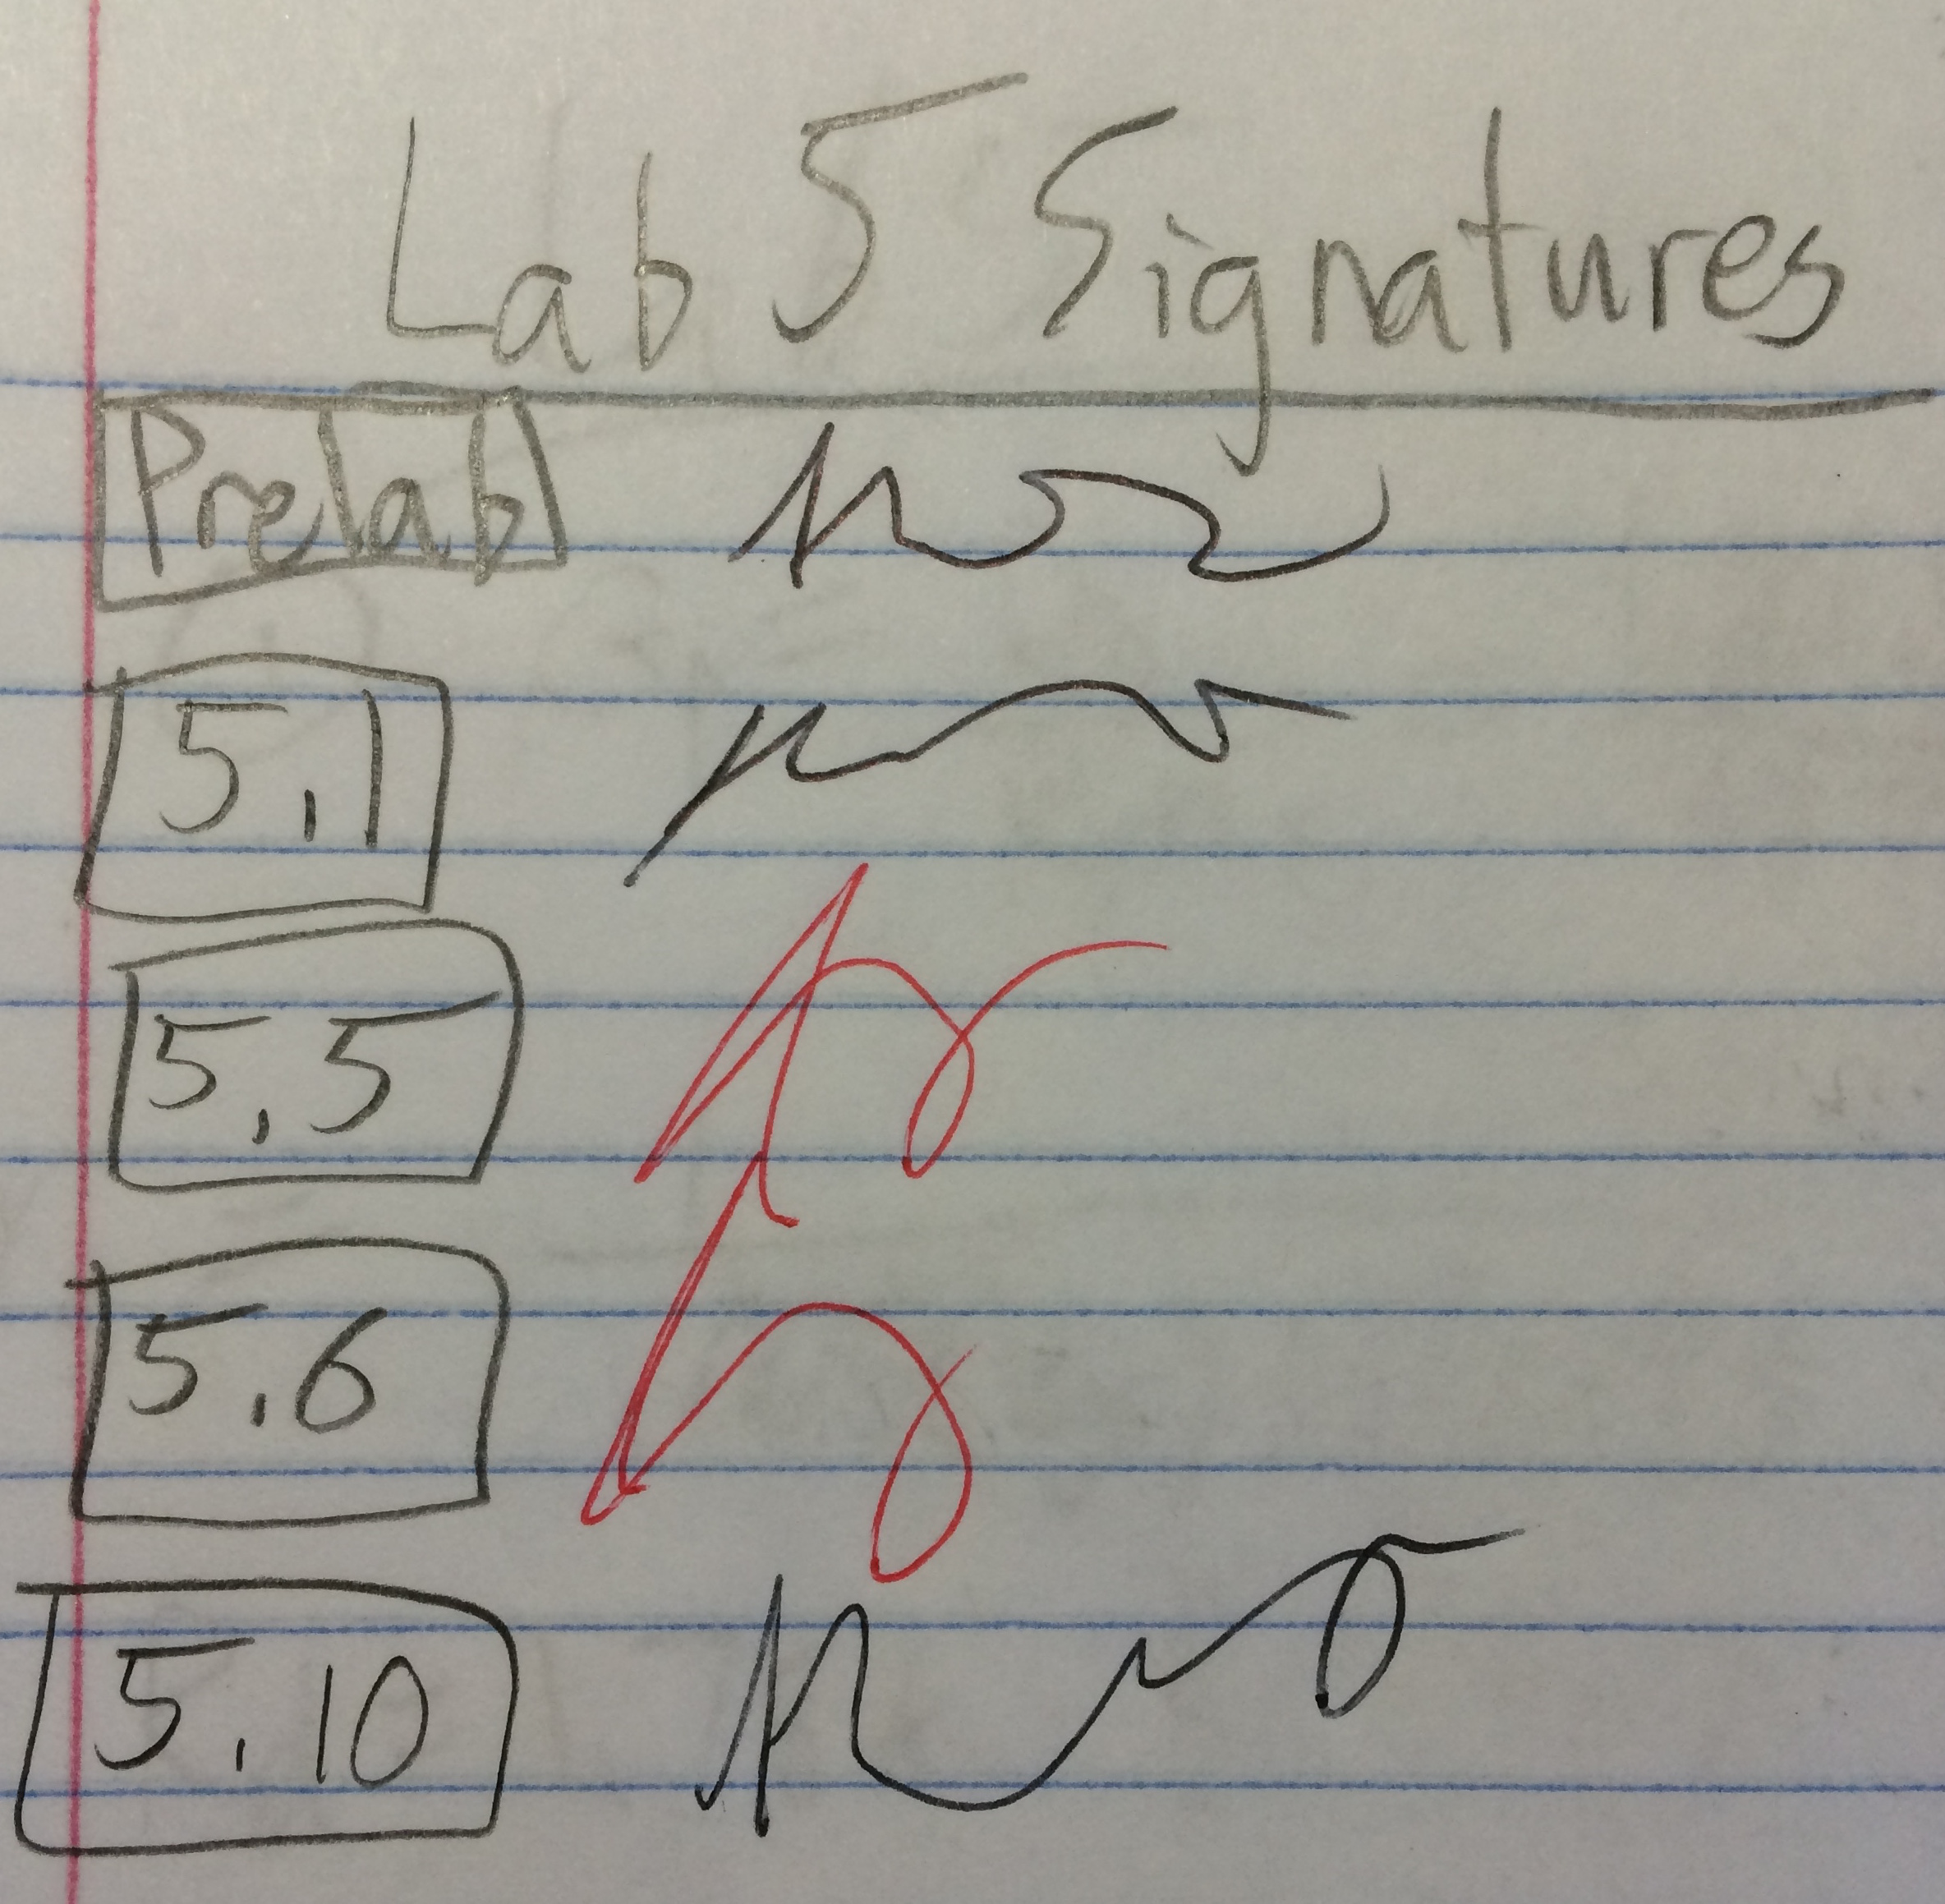
\includegraphics[scale = 0.1]{IMG1.jpg}$
\end{center}

\bibliography{joshbib}{}
\bibliographystyle{plain}

\end{document}
